%%% SETUP %%%
\documentclass{article}
\usepackage[utf8]{inputenc}
\usepackage{titling} %Subtitle Package
\usepackage{setspace}
\usepackage{hyperref}
\setcounter{secnumdepth}{0} %Table of contents without numbers

%  Subtitle Setup %
% https://tex.stackexchange.com/questions/50182/subtitle-with-the-maketitle-page
\newcommand{\subtitle}[1]{%
  \posttitle{%
    \par\end{center}
    \begin{center}\large#1\end{center}
    \vskip0.5em}%
}

% Graphics %
% https://en.wikibooks.org/wiki/LaTeX/Importing_Graphics
\usepackage{graphicx}
\graphicspath{ {./} }

%Double Spacing%
\doublespacing

%  Title Page Setup %
\title{Learning Journal}
\subtitle{FOAR705 2019}
\author{Matthew Clark}
\date{\vspace{-5ex}} %Used to remove date when using \maketitle%
% /Title Page Setup %
%%%%% /SETUP %%%%%
%%%%%  Title Page %%%%%
\begin{document}
\maketitle
%%%%% /Title Page %%%%%
%%%%%  Table of Contents %%%%%
\newpage
\tableofcontents
%%%%% /Table of Contents %%%%%
%%%%%%%%%%%%%%%%%%%%%%%%%%%%%%%%%%%%%%%%%%%%%%%%%%%%%%%%%
%%%%%%%%%% New Entry %%%%%%%%%%
\newpage
\begin{center}
\section{Week 1 Assignment}
Week 1
\end{center}
\noindent
\textbf{Objective:} To attempt to download and restore a backup from 6 months or older\\
\textbf{Action:}
\begin{enumerate}
    \item Identify what file I want to back up
    \begin{itemize}
        \item I will be attempting to restore an old Ableton Live project from 4 years ago from my Google Drive
    \end{itemize}
    \item Open Google Drive, locate the file
    \item Download the file
    \item Open the file in Ableton and see how it works
\end{enumerate}
\textbf{Errors:} No errors were encountered. \\
\textbf{Results:} I was able to successfully download and open a file from 4 years ago. However, it does highlight that my current backup system (Google Drive) will synchronize the most recent item version and replace an older version, meaning I have a backup, but I have no version control within my backup. This will be a point of action for future me to explore down the line.
%%%%%%%%%% New Entry %%%%%%%%%%
\newpage
\section{Data carpentry Exercises 1 \& 2: Formatting Data}
\subsection{Task 1: Analyzing Messy Data}
\textbf{Objective:} To work through the first exercise in \textit{01: Format Data} by using examples from \textit{02: Common Mistakes}.
\newline
\textbf{Action:}
\begin{enumerate}
    \item Download the messy data
    \item Open up the data in a spreadsheet program
    \item Analyze what is wrong with the spreadsheet and discuss ways to clean up the the two tabs in order to put them into one spreadsheet
\end{enumerate}
\textbf{Analysis:}
\begin{itemize}
    \item Using multiple data tables within 1 spreadsheet
    \begin{itemize}
        \item Both tabs contain multiple tables. The issue with this is that the computer can correlate columns and rows from different tables to mean the same thing, and if they contain the wrong data, this will end up with a miscorrelation or an error.
        \item \textbf{To solve:} Have all corresponding data written out such that there are no tables and create extra columns for different variables
    \end{itemize}
    \item Using multiple tabs per spreadsheet
    \begin{itemize}
        \item This can cause issues with particular types of data analysis software, and is preferred to avoid this
        \item \textbf{To Solve:} Place all data in one spreadsheet with extra columns for different variable types which correspond to the different countries used.
    \end{itemize}
    \item Putting more than one type of variable per column
    \begin{itemize}
        \item Both tabs have columns which use different data types or variables per column. In the \textit{Mozambique} tab, the livestock count contain the number of livestock, and what type, with no correlation between what the number means in relation to it. There is also a comment in the Water table which states (only in summer), which will confuse analysis software. In the \textit{Tanzania} tab, the livestock table contains columns with both numerical values and boolean values, which causes both confusion for the human reading and the computer analysing the data
        \item \textbf{To Solve:} Create new columns such that each column corresponds to only 1 variable. As for the \textit{Tanzania} data, create 2 columns, one for \textit{animalsObversed} and use a boolean, and a \textit{numOfAnimals} used if the animals were counted, left blank if the data is missing/incomplete as a NULL value.
    \end{itemize}
    \item Zeros and Nulls
    \begin{itemize}
        \item Zeros should be used when there is a 0 observation result, and a NULL should be used when there is missing or incomplete data, and the 2 should not be mixed up. The best representation of NULL is a blank space, as other forms, such as negative numbers, can be misinterpreted as a negative value. The \textit{Mozambique} data contains both negative values, such as '-99' and '-999', while also using blanks and zeros. The \textit{Tanzania} data uses blanks, however due to the amount of blanks used, it is hard to gather whether or not the researcher intended them to be NULLS or zeros
        \item \textbf{To Solve:} Replace negative values as blank spaces, and use zeros to correspond to zero observations. 
    \end{itemize}
    \item Variation in Spelling
    \begin{itemize}
        \item If a computer program is reading the data, it will distinguish a misspelling as a different type of data. For example, in the \textit{Mozambique} data, the researcher misspells 'earth' as 'errth' a couple of times.
        \item \textbf{To Solve:} Clean up data so that all words are spelt correctly
    \end{itemize}
    \item Variations in variable recording
    \begin{itemize}
        \item If a computer program is reading the data, variations in the variable recording could create issues such as errors or different categorization of variables. Most notably is the \textit{Mozambique} 'plots' table, which uses both 'n' and 'no' to mean the same thing, while also using 'yes' and 'yes (only in summer)', which will cause confusion. There is also a number '1', which adds to the confusion.
        \item \textbf{To Solve:} Make sure all variables are denoted the same way; if using a boolean, then do not use numbers as well. Use an extra column to denote if applicable to a particular season.
    \end{itemize}
    \item Using formatting to convey data
    \begin{itemize}
        \item A computer cannot read a coloured cell easily, and if a custom script is designed to accomodate for this, cross-compatibility will be compromised
        \item \textbf{To Solve:} Use a new column to denote a sub-variable instead of a colour to denote a comment
    \end{itemize}
    \item Merging Cells
    \begin{itemize}
        \item The headings used for the tables are located in merged cells. This can cause issues for data analysis software.
        \item \textbf{To Solve:} Do not use merged cells. Rather, create another column which denotes what you are looking at (Eg: typeOfObservation - plot, water, livestock, floorType etc)
    \end{itemize}
    \item Spaces used
    \begin{itemize}
        \item Spaces can cause issues with some programs. It is better to use camelCase of underscores to avoid this issue.
        \item \textbf{To Solve:} Change all cells with spaces between words with camelCase or underscores (eg: floorType, wallType etc)
    \end{itemize}
    \item Special Characters
    \begin{itemize}
        \item Special characters such as parenthesis or asterisks may have a \\
        special meaning in particular programs, causing an unintended input/output. Best to avoid these
        \item \textbf{To Solve:} Treat comments in parenthesis or asterisks as variables and add them into new, different columns.
    \end{itemize}
\end{itemize}
\textbf{Errors:} No errors were involved when downloading or opening the files, or exploring the Data Carpentry website.
\newline
\textbf{Result:} Gained new knowledge about what not to do when recording data in a spreadsheet, and ways to clean up existing data.
%
\subsection{Task 2: Metadata}
%
\textbf{Objective:} To analyse the Clean spreadsheet and discuss useful types of Metadata to improve readability (from \textit{01: Formal Data}.)
\newline
\textbf{Action:}
\begin{enumerate}
    \item Download the clean data
    \item Analyse and record different types of Metadata I would include for this spreadsheet
\end{enumerate}
\textbf{Analysis:}
\begin{itemize}
    \item Some of the keyID's are out of order, any reason to that?
    \item Where abouts are the villages located?
    \item What was the specific questions asked
    \item What is meant by 'muddaub' and 'burntbricks'
    \item Define what is meant by 'membAssoc', 'affectConflict' and 'livCount'
    \item Define what time period 'noMeals' is \\ referring to (Per person, daily, weekly?)
    \item Define what is meant by 'instanceID'
\end{itemize}
\textbf{Errors}: No errors encounted when download or opening the text file, or when analysing the data. The only warning when opening the .csv format is that possible data loss may occur when the workbook is saved in this format. I assume that because the .csv format does not account for formatting, unlike an excel format, that if the data is written out correctly, this is not an issue, however any incorrect formatting could result in a loss of data.\\
\textbf{Results:} In looking into this file, it is good to realise that your data will be read by other people, and having a Metadata text file to explain all the shorthands and the way you gathered your data is crucial for others to understand your data structure. 
\newpage
%%%%%%%%%% New Sub-Entry %%%%%%%%%%
\section{Analysing other data from similar fields}
\textbf{Objective:} To explore and analyse other datasets from my field for potential issues in their formatting\\
\textbf{Action:}
\begin{enumerate}
    \item Research potential datasets used in the analysis of modern electronic music
    \item Download, unzip, and open the .csv files in excel
    \item Look through the data set and analyse the fields for any potential issues
\end{enumerate}
\textbf{Errors:} There were no issues that occured when researching, downloading, unzipping, and opening these files. \\
\textbf{Results:}
\begin{itemize}
    \item First data set is titled "DJ Mag Top 100 History Dataset" and was \\ retrieved from https://www.kaggle.com/koki25ando/dj-mag-top-100-\\history-dataset
    \begin{itemize}
        \item  The data set was set up correctly. The only issue was the character ë found in Tiësto's name, and because it is a special character with an umlaut, it gets converted to TiÃ<sto, which also has special characters, and may cause further issues for extra programs
        \item \textbf{To Solve:} Anglicize the name to be Tiesto to avoid any reading issues, and make a note in the Metadata.
    \end{itemize}
    \item Second data set is titled "FMA: A dataset for musical analysis" and was retrieved from https://github.com/mdeff/fma
    \begin{itemize}
        \item Overall, the data set was all laid out correctly. I did spot a question mark in box AJ164 instead of having a blank.
    \end{itemize}
    \item Last data set is titled "Pitchfork's reviews(aka musical's genres battle)" and was retrieved from \\https://www.kaggle.com/bcyphers/pitchfork-reviews/
    \begin{itemize}
        \item I could not find any issue with this data set other than the conversion of special characters under 'content' as it was scrapped off the web. I do like how it has categorised dates as having a column for each variable of the date (One for day, one for month, one for year).
    \end{itemize}
\end{itemize}
%%%%%%%%%% New Entry %%%%%%%%%%
\newpage
\section{LaTeX in Overleaf}
\textbf{Objective:} To document my first use of Overleaf, including useful commands to remember later, and errors that were encountered
\newline
\textbf{Action:} Commands that were used so far for future me to remember include:
\begin{itemize}
    \item center: Centre Text
    \item section*: New, unnumbered section
    \item date: Write the specified date
    \item textbf: Bold
    \item textit: Italics
    \item newline: Tells LaTeX to start a new line. Use this with caution.
    \item enumeration: Ordered List. Can be nested.
    \item itemize: Unordered List. Can be nested.
    \item vspace: Creates a vertical space. Useful for formatting. Use mm.
    \item Percentage sign: Comment in code.
    \item newpage: Puts the next text onto a new page
\end{itemize}
\textbf{Errors:} I encountered a few errors so far in using Overleaf:
\begin{itemize}
    \item Formatting code manually (Adding in extra tabs)
    \begin{itemize}
        \item While this didn't break compilation, it did pop up and ask why this was done?
        \item \textbf{Solved by:} Removing any extra tabs in the coding. Error went away
    \end{itemize}
    \item Used the Ampersand symbol in text instead of the word 'and'
    \begin{itemize}
        \item The ampersand symbol did not display as text. The symbol is used as a function in the itemize environment.
        \item \textbf{Solved by:} Replacing it with the word 'and'. You can also use a backslash before the ampersand symbol to avoid it disappearing or causing an error.
    \end{itemize}
    \item Using an underscore
    \begin{itemize}
        \item The underscore cannot be used unless in Math mode.
        \item \textbf{Solved by:} When noting examples, \\ I used camelCase instead. Learned that you can use a backslash before the underscore to use it as plain text.
    \end{itemize}
    \item Overfull hbox
    \begin{itemize}
        \item Found this to occur periodically. According to overleaf, "Overfull hbox messages tell you that some line sticks out over the right margin".
        \item \textbf{Solved by:} There were various manual ways of adjusting hboxes. My quick fix was to use a double backslash as a line break to manual divide the line such that overleaf could not complain that it couldn't fit the entire line in. Will see in future if this quick fix over time breaks the system.
    \end{itemize}
    \item Underfull hbox
    \begin{itemize}
        \item Found that when I incorrectly used the newline function, it would spit out this error. Overleaf states "Underfull hbox messages tell you that some line is poorly typeset (or that you've improperly used newline to leave a vertical space (for example, typing two newline in a row);"
        \item \textbf{Solved by:} checking where I have incorrectly used a double backslash or newline. Error went away
    \end{itemize}
    \item Being able to type in a command as plain text and have it not execute
        \begin{itemize}
            \item If i wanted to type in a command for the previous dot points, it would execute instead of staying as plain text
            \item \textbf{Solved by:} Found out about the 'verbatim' command. Will utilize next time.
        \end{itemize}
    \item Having vspace and newline commands not interact properly, causing the line after to space out
        \begin{itemize}
            \item \textbf{To Solve:} Follow this ordering (vspace first):
            \begin{verbatim}
                \vspace{5mm}
                \newline
            \end{verbatim}
        \end{itemize}
\end{itemize}
\textbf{Analysis:} New TeX commands that were found and used include:
    \begin{itemize}
        \item Useful packages:
        \begin{itemize}
            \item \verb|\usepackage{titling}|: Useful for creating subtitles
            \item \verb|\usepackage{setspace}|: Used for setting line spacing to normal, 1.5, or double spacing
        \end{itemize}
        \item New Commands:
        \begin{itemize}
            \item \verb|\onehalfspacing|: Set the line spacing to 1.5
            \item \verb|\verb|: Typing out a single command without using a verbatim block
            \item \texttt{Ctrl + B; Ctrl + I; Ctrl + U}: Shortcuts for \verb|\textbf{}| etc.
            \item \verb|texttt{}|: Typewriter font
        \end{itemize}
    \end{itemize}
\textbf{Results:} Was able to research about errors and ways of formatting LaTeX so that:
\begin{enumerate}
    \item Next time, I can solve errors that I have so far encountered quickly without having to research them
    \item Be able to use the \& and \_ symbols without dropping errors or disappearing
    \item Use the verbatim command to document new commands in full text.
\end{enumerate}
%%%%%%%%%% New Entry %%%%%%%%%%
\newpage
\section{Data Carpentry Exercise 3: Dates as Data}
\textbf{Objective:}
\begin{enumerate}
    \item To convert a dd/mm/yyyy column into 3 columns for each date variable
    \item To add a new date entry and analyse the result of the year column
\end{enumerate}
\textbf{Action:}
\begin{enumerate}
    \item Download and open SAFI\_dates.xlsx
    \item Create 3 new columns: day; month; year
    \item Change the formatting of these columns from \textit{dates} to \textit{number}
    \item Use Excel's in-built functions to extract each variable\\ (\verb|=DAY(); =MONTH(); =YEAR();|)
    \item Add the date \textit{17/11} to the end of \textit{interview\_date} and analyse the results
\end{enumerate}
\textbf{Analysis}
\begin{itemize}
    \item Was relatively simple to convert \textit{interview\_date} to its new columns
    \item When I entered the new date without a year, it automatically changed it to the current year (\textit{2019}), which could be an issue if the researcher forgot to enter the year.
\end{itemize}
\textbf{Errors:}
\begin{itemize}
    \item I used the Excel functions before formatting the cell's data type to \textit{number}, and what it would do was display a date with the correct variable I was converting, and setting the rest of the variables to the default.
    \begin{itemize}
        \item Example: \verb|=DAY(17/11/2016)| turns into:\\ \textit{17/01/1900}
    \end{itemize}
    After realizing what I had done and changed the format to \textit{number}, it was good to know how it functioned.
\end{itemize}
\textbf{Result:}
\begin{itemize}
    \item Was able to create 3 new columns per date variable, and analyse a date input with no year attached to it.
\end{itemize}
%%%%%%%%%% New Entry %%%%%%%%%%
\newpage
\begin{center}
\section{Data Carpentry Exercise 4: Quality Assurance}
\end{center}
\textbf{Objective:} To utilize Excel's ability to restrict the input of a certain cell to a particular form of data or data range \\
\textbf{Action:}
\begin{enumerate}
    \item Download and open a fresh \verb|SAFI_clean.csv| file
    \item Select an applicable column to restrict its input range, and use Excel's \verb|Data Validation| tool to execute it.
    \item Select an applicable column to restrict its input set to a list, and use Excel's \verb|Data Validation| tool to execute it.
\end{enumerate}
Excel's \verb|Data Validation| is located: \begin{center}
\verb|Data > Data Tools > Data Validation|
\end{center}
\textbf{Errors:}
No errors occurred during this exercise.\\
\textbf{Result:}
\begin{itemize}
    \item I was able to set up a range restriction on \verb|years_lived| to \\\verb|between 0 - 123| alongside an error message and tested it out, which worked as expected.
    \item I was able to set up a list restriction on \verb|memb_assoc| to \verb|yes, no, NULL| alongside an error message and tested it out, which worked as expected
\end{itemize}
%%%%%%%%%% New Entry %%%%%%%%%%
\newpage
\begin{center}
\section{Data Carpentry Exercise 5: Exporting Data}
\end{center}
\textbf{Objective:} To save a file in Excel as a \verb|.csv|.\\
\textbf{Action:}
\begin{enumerate}
    \item In excel, go to \verb|File > Save As|
    \item Under \verb|Format|, select \verb|Comma Separated Values|.
    \item Hit Save
    \item Open up the file in Notepad++ and observe the result
\end{enumerate}
\textbf{Analysis:} When opening the document in Notepad++, its easy to observe how a \verb|.csv| functions, and even without special parsing software, you can still understand the general gist of the data presented before you. Its universality means long-time backwards compatibility and minimises potential data loss or data corruption.\\
\textbf{Errors:} No errors were encountered.\\
\textbf{Results:} Was able to export a file as a .csv, and was able to open it in Notepad++.
%%%%%%%%%% New Entry %%%%%%%%%%
\newpage
\begin{center}
\section{Further Analysis of Overleaf}
22 August 2019
\end{center}
\textbf{Objective:} To document further errors encountered when working in Overleaf/LaTeX. \\
\textbf{Errors:} 3 added errors I have encountered thus far include:
\begin{itemize}
    \item The \verb|=| disappears when used as text; \verb|\=| doesn't help.
    \item The use of \verb|_| throws an error (Can only be used in MATH\_MODE; \verb|\_| seems to resolve this error
    \item There was a section where I accidentally used \verb|\(|, which threw an error about MATH\_MODE; removing it fixed the issue.
\end{itemize}
\textbf{Analysis:}
\begin{itemize}
    \item \verb|=| is a function used in MATH\_MODE;
    \item \verb|_| is a function used in MATH\_MODE;
    \item After some research, you can initialize MATH\_MODE by using the \verb|\( \)| braces.
\end{itemize}
\textbf{Results:} Discovered some more about LaTeX's MATH\_MODE, and have \\started using \verb|\verb| more to overcome errors when using special characters as text.
%%%%%%%%%% New Title %%%%%%%%%%
\newpage
\title{Unix Shell Exercises + Overleaf notes}
\maketitle
%%%%%%%%%% New Entry %%%%%%%%%%
\newpage
\section{Unix Shell Exercise 1: Setup \& Introduction}
\textbf{Objective:} To read through and understand the setup and introduction to the Unix Shell\\
\textbf{Action:}
\begin{enumerate}
    \item Open Bash in Ubuntu for Windows, as it was already installed on my computer from my undergraduate degree
    \item Test out the \verb|$ls| command
\end{enumerate}
\textbf{Errors:} Unable to access my C:/ drive. Was able to move my current directory through \verb|cd /mnt/c|. From there, \texttt{ls} displayed my files in my C drive.\\
\textbf{Analysis:} Luckily, I had already altered my computer to run Linux within windows so I had instant access to the shell.\\
\textbf{Result:} Successfully opened Bash \& tested out the first command
%%%%%%%%%% New Entry %%%%%%%%%%
\newpage
\section{Unix Shell Exercise 2: Navigating Files and Directories}
%
\subsection{Task 1: Exploring More ls Flags}
%
\textbf{Objective:} To test out and analyse the given flags for \texttt{ls}\\
\textbf{Action:} Run the following commands:
\begin{verbatim}
    \item \verb|ls -l|
    \item \verb|ls -l -h|
\end{verbatim}
\textbf{Errors:} Mistook \verb|-l| for \verb|-1| and didn't display what I wanted. Realised and changed the flag. Worked after that.\\
\textbf{Analysis:} When comparing \verb|ls|; \verb|ls -l| \& \verb|ls -l -h|, 
\begin{enumerate}
    \item \verb|ls -l| displayed the following: \\
    \verb|-rwxrwxrwx 1 root root    13076 Jan 17  2019|
    \item \verb|ls -l -h| displayed the following: \\
    \verb|-rwxrwxrwx 1 root root  13K Jan 17  2019|
\end{enumerate}
By the looks of things, it will display the file size and the date last modified. \verb|-h|, according to \textit{Solutions}, stands for \textbf{H}uman Readable, and converts the file size to a more readable format. It also states the file type \& the links back to the root directory.\\
\textbf{Result:} Was able to test out \verb|ls -l| \& \verb|ls -l -h|.
%
\subsection{Task 2: Listing Recursively and By Time}
%
\textbf{Objective:} To execute and analyse some \texttt{ls} flags associated with recursion and time\\
\textbf{Action:} Test out the following flags:
\begin{enumerate}
    \item \verb|ls -R|: List recursively
    \item \verb|ls -t|: List by time last changed
    \item \verb|ls -R -t|: Test out what order this is sorted in
\end{enumerate}
\textbf{Errors:} No errors were encountered.\\
\textbf{Analysis:} When comparing \verb|ls -R|; \verb|ls -l -t|; \verb|ls -l -R -t|:
\begin{enumerate}
    \item \verb|ls -R| went through every single file in every single sub-directory in about 10 seconds
    \item \verb|ls -l -t| listed the files/folders in my directory by time last changed, and when used in conjunction with \verb|-l|, I could see the result
    \item \verb|ls -l -R -t|: Listed every single file in every sub-directory by time last changed, presented in long form
\end{enumerate}
\textbf{Result:} Was able to test out \verb|ls -R| \& \verb|ls -t|;
%
\subsection{Task 3: Absolute vs. Relative Path }
%
\textbf{Objective:} To analyse the correct way to move the current directory around.\\
\textbf{Action:} Starting from \texttt{/Users/amanda/data}, analyse what command will get her back to \texttt{/Users/amanda}?\\
\textbf{Errors:} No errors were encountered.\\
\textbf{Analysis:} Amanda can use the following:
\begin{enumerate}
    \item \verb|cd ~|: \verb|~| stands for the home directory, so \verb|cd ~| navigates to the home directory.
    \item \verb|cd ~/data/..|: Would navigate to home, down to data, then back up to home. Over-complicated, but it works.
    \item \verb|cd|: Shortcut to go back home
    \item \verb|cd ..|: Moves back up one level, which is home.
\end{enumerate}
\textbf{Result:} Was able to analyse and be able to move directory around using path commands.
%
\subsection{Task 4: Relative Path Resolution}
%
\textbf{Objective:} To trace through a relative path given our present working \\directory.\\
\textbf{Action:} Given the file system diagram, if \verb|pwd| displays \verb|/Users/thing|, what will '\verb|ls -F ../backup|' display?\\
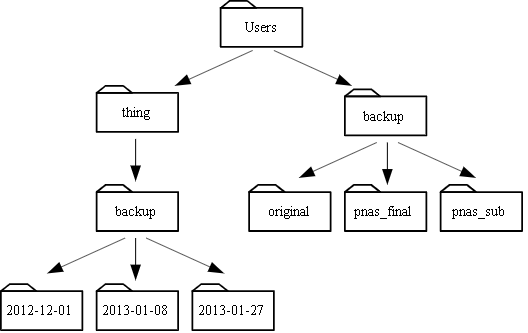
\includegraphics[width=11cm]{filesystem.png}
\begin{center}
    \texttt{https://swcarpentry.github.io/shell-novice/02-filedir/index}\\
\end{center}
\textbf{Errors:} No errors were encountered.\\
\textbf{Analysis:}
\begin{itemize}
    \item \verb|ls -F| lists files with their file type
    \item \verb|..| brings the directory up a level
    \item \verb|/backup| navigates the directory down a level to the folder \verb|backup|
\end{itemize}
Hence, it would display:\\
\verb|original/ pnas_final/ pnas_sub/|\\
\textbf{Result:} Was able to correctly identify the result of the command \\\verb|ls -F ../backup|
%
\subsection{Task 5: ls Reading Comprehension}
%
\textbf{Objective:} To trace through a relative path given our present working directory.\\
\textbf{Action:} Using the same file system diagram, if \texttt{pwd} displays \texttt{/Users/backup}, and \texttt{-r} tells \texttt{ls} to display things in reverse order, what command(s) will result in the following output:\\
\verb|pnas_sub/ pnas_final/ original/|\\
\textbf{Errors:} No errors were encountered.\\
\textbf{Analysis:} 
\begin{enumerate}
    \item Because \verb|-r| will list the folders backwards, which is what the given list is listed as, and \verb|-F| will display the file type, which are folders, the correct command would be \verb|ls -r -F|. 
    \item \verb|ls -r -F /Users/backup| would also work, but is unnecessary as we are already in backup.
\end{enumerate}
\textbf{Results:} Successfully identified the correct commands given the objective.
%%%%%%%%%% New Entry %%%%%%%%%%
\newpage
\section{Unix Shell Exercise 3: Files and Directories}
%
\subsection{Task 1: Creating Files}
%
\textbf{Objective:} Test out the \verb|touch| command and create a blank text file. Analyse what happened, how big is the file, and why would you want to use \verb|touch|?
\textbf{Action:}
Executed the command \verb|touch my_file.txt|\\
\textbf{Errors:} No errors were found\\
\textbf{Analysis:} \verb|touch| creates a new file, in this case a text file, without opening the editor, unlike \verb|nano|. The file is 0 bytes in size. According to the \textit{solution}, this is helpful when programs require a blank file to already be generated so it can output data.\\
\textbf{Results:} Successfully identified what the \verb|touch| command did. Had to use the \textit{Solution} to find out why.
%
\subsection{Task 2: Moving to the Current Folder}
%
\textbf{Objective:} Move 2 files from the current directory to another folder shared by the folder above.\\
\textbf{Action:} Fill in the blanks:\\\verb|$ mv ___/sucrose.dat ___/maltose.dat|\\
\textbf{Errors:} Not applicable\\
\textbf{Analysis:} \verb|mv| will move the located file to the current directory. To locate the files, we must move up a level and then access the old folder \verb|analysed/|. Hence, we execute the command:\\
\verb|mv ../analyzed/sucrose.dat ../analyzed/maltose.dat|.\\
\textbf{Results:} Correctly identified the way to move a file from one folder to another folder using the shell.
%
\subsection{Task 3: Renaming Files}
%
\textbf{Objective:} To identify how to rename a file.\\
\textbf{Action:} Analyse the 4 options and determine which is the correct command.\\
\textbf{Errors:} Not applicable\\
\textbf{Analysis:} To rename a file, we use the \verb|mv| command in the following way:\\\verb|mv statstics.txt statistics.txt|.\\
\textbf{Results:} Correctly identified the right way to rename a file.
%
\subsection{Task 4: Moving and Copying}
%
\textbf{Objective:} To analyse the line-by-line code and identify the result\\
\textbf{Action:} Analyse the code and pick a solution:\\ \verb|proteins-saved.dat recombine|
\textbf{Errors:} The correct answer was \verb|recombine|.\\
\textbf{Analysis:} I forgot that the \verb|..| meant move up a level from where the directory is, not where the file is located, and hence we copied the file above the current directory. Hence, the correct answer was \verb|recombine|.\\
\textbf{Result:} Picked the wrong answer, and analysed the correct answer in \textit{solution}.
%
\subsection{Task 5: Using rm Safely}
%
\textbf{Objective:} To analyse what \verb|-i| does when using the remove command\\
\textbf{Action:} Use the remove command to remove a file:\\\verb|rm -i thesis_backup/quotations.txt|\\
\textbf{Errors:} No errors encountered\\
\textbf{Analysis:} Using the \verb|-i| flag gives us a prompt before removing the file. The shell doesn't have a recycling bin like windows, and hence once a file is removed, it is gone forever (mostly).//
\textbf{Result:} Identify the use of \verb|rm -i|
%
\subsection{Task 6: Copy with Multiple Filenames}
%
\textbf{Objective:} To identify the results when copying multiple files in the same \verb|cp| command\\
\textbf{Action:}
\begin{enumerate}
    \item Explain what happens when the following command is executed:\\
    \verb|$ cp amino-acids.txt animals.txt backup/|
    \item Explain what happens when the following command is executed:\\
    \verb|$ cp amino-acids.txt animals.txt morse.txt |
\end{enumerate}
\textbf{Errors:} No errors were encountered.
\textbf{Analysis:}
\begin{enumerate}
    \item When there are multiple files in the same \verb|cp| command, the last argument is treated as the destination, and the files listed beforehand are copied there. In this case, \verb|amino-acids.txt| \& \texttt{animals.txt} copied to \verb|backup/|.
    \item Because the last argument is treated as the destination, the command would throw an error stating that \texttt{morse.txt} is not a destination.
\end{enumerate}
\textbf{Result:} Learned about copying multiple files and the correct syntax needed to execute \texttt{cp} without throwing an error.
%
\subsection{Task 7: List filenames matching a pattern}
%
\textbf{Objective:} To identify the correct use of wildcards\\
\textbf{Action:} Using the \texttt{molecules/} directory, what command produces the output \texttt{ethane.pdb methane.pdb}?\\
\textbf{Errors:} No errors were encountered.
\textbf{Analysis:} One has to remember that \verb|*| means \textit{zero or more characters}, where as \verb|?| is only a single character wildcard. However, I was able to identify that \verb|ls *t??ne.pdb| was the correct command.\\
\textbf{Result:} Was able to analyse and pick the corrent command for the expected output.
%
\subsection{Task 7: More on wildcards}
%
\textbf{Objective:} To identify the correct use of wildcards for the intended output
\textbf{Action:} Fill in the blanks to correctly output the intended output\\
\textbf{Errors:} No errors were encountered.\\
\textbf{Analysis:} \verb|$ cp *calibration.txt backup/calibration| would copy all calibration files to \verb|backup/calibration|.\\
\verb|$ cp 2015-11-* send_to_bob/all_november_files/| would copy all files \\made in November to \verb|send_to_bob/all_november_files/|.\\
\verb|$ cp *-*-23-dataset* send_to_bob/all_datasets_created_on_a_23rd/|\\ would copy all datastes made on the 23rd to \\\verb|send_to_bob/all_datasets_created_on_a_23rd/|. It could be simplified further to \verb|*-23-dataset*|\\
\textbf{Result:} Was able to correctly identify the correct command for the intended output, however my third answer could be simplified further.
%
\subsection{Task 8: Organising Files and Directories}
%
\textbf{Objective:} To figure out the correct way to move multiple items into a \\subdirectory\\
\textbf{Action:} If \verb|ls -F| resulted in the output:\\ \verb|analyzed/  fructose.dat    raw/   sucrose.dat|, identify the correct \\command to move the \verb|.dat| files into \verb|analyzed/|?\\
\textbf{Errors:} No errors were encountered\\
\textbf{Analysis:} Inferring from the previous tasks, I identified the following command would work:\\
\verb|$ mv fructose.dat sucrose.dat analyzed/|\\
However, this could be further simplified by using a wildcard:\\
\verb|$ mv *.dat analyzed/|\\
\textbf{Result:} Correctly moved 2 files into a subdirectory, however discovered\\ my command could've been simplified by using a wildcard.
%
\subsection{Task 9: Reproduce a folder structure}
%
\textbf{Objective:} To reproduce a folder layout using the \texttt{mkdir} command.\\
\textbf{Action:} From 4 options, pick the correct command(s) which results in the following folder layout:
\begin{verbatim}
    2016-05-20/
    |- data
        |-- processed
        |-- raw
\end{verbatim}
\textbf{Errors:} No errors were encountered\\
\textbf{Analysis:} I correctly picked the 2 correct ways by creating the directory before creating the sub-directories and so forth. I was not sure about the syntax, but you can do the following:
\begin{itemize}
    \item \verb|mkdir 2016-05-20/data| to create the subdirectory \verb|data| if the level above was already created.
    \item \verb|mkdir processed raw| will create 2 folders at the same time in the current directory.
\end{itemize}
\textbf{Results:} Correctly analysed how to create folder structures within the Unix shell.
%%%%%%%%%% New Entry %%%%%%%%%%
\newpage
\section{Syntax \& Commands for the Unix Shell}
\textbf{Objective:} To document helpful syntax and commands learned so far when using the Unix shell.\\
\textbf{Action:}
\begin{itemize}
    \item Shell Syntax
    \begin{itemize}
        \item \verb|/|: Root or Directory
        \item \verb|@|: Link
        \item \verb|*|: Executable
        \item \verb|~|: User's home directory
    \end{itemize}
    \item Shell Commands \& Flags
    \begin{itemize}
        \item \verb|pwd|: Present working directory
        \item \verb|ls|: List sub-directories
        \begin{itemize}
            \item \verb|-a|: Show all files including hidden files
            \item \verb|-F|: Show file type by adding a char to entry
            \item \verb|-l|: Long format: Show extra information
            \item \verb|-R|: List directory tree recursively
            \item \verb|-s|: List by file size
            \item \verb|-t|: List by time \& date
        \end{itemize}
        \item \verb|cd|: Command directory
        \begin{itemize}
            \item \verb|cd <folder>|: Used to move the working directory to that folder
            \item \verb|cd ..|: Move up a level
        \end{itemize}
        \item \verb|mkdir|: Make a directory
        \item \verb|touch|: Generate a new file.
        \item \verb|nano|: Generate a new text file and open it in \textit{nano}
        \item \verb|mv|: Move the located file to the current directory. Can also be used to overwrite/rename.
        \begin{itemize}
            \item \verb|-i|: Asks you for confirmation before moving.
        \end{itemize}
        \item \verb|cp|: Copy the located file to the current directory.
        \begin{itemize}
            \item \verb|-r| Used to copy a directory and all its contents recursively.
        \end{itemize}
        \item \verb|rm|: Remove the located file.
        \begin{itemize}
            \item \verb|-i|: Prompt the user before removing file.
        \end{itemize}
        \item \verb|*|: Zero or more character wildcard.
        \begin{itemize}
            \item \verb|?|: Single char wildcard. Can be used multiple times for multiple char's.
        \end{itemize}
    \end{itemize}
    \item Keyboard Shortcuts
    \begin{itemize}
        \item \verb|Ctrl+L|: Clear the shell window
    \end{itemize}
\end{itemize}
%%%%%%%%%% New Entry %%%%%%%%%%
\newpage
\section{Unix Shell Exercise 4: Pipes and Filters}
\subsection{Task 1: What does \texttt{sort -n} do?}
\textbf{Objective: To understand what the \texttt{sort} command and the \texttt{-n} flag do}\\
\textbf{Action:} Analyse what happens when you sort a list of 6 numbers by \texttt{sort}, then \texttt{sort -n}, and compare the 2.\\
\textbf{Errors:} No errors were encountered.\\
\textbf{Analysis:} When using \texttt{sort}, it will sort the numbers vertically, one integer at a time (essentially by ASCII alphabetically) \texttt{sort -n} will treat each number as a whole integer, and sort by integer value instead.\\
\textbf{Result:} Learned what \texttt{sort} and \texttt{sort -n} do.
%
\subsection{Task 2: Overwriting vs. Appending}
%
\textbf{Objective:} To distinguish the difference between \verb|>| and \verb|>>|\\
\textbf{Action:}
\begin{enumerate}
    \item Execute the command: \verb|echo hello > textfile01.txt|
    \item Execute the command: \verb|echo hello >> textfile02.txt|
    \item Repeat Step 1 \& 2
    \item Analyse what happens using \texttt{nano}
\end{enumerate}
\textbf{Errors:} No errors were encountered\\
\textbf{Analysis:} The \verb|>| command will overwrite a file with the same name. \verb|>>| will instead append the file.\\
\textbf{Result:} Learned the difference between \verb|>| and \verb|>>|
%
\subsection{Task 3: Appending Data}
%
\textbf{Objective:} To analyse the result when using \texttt{head}, \texttt{tail}, and \verb|>>|\\
\textbf{Action:} Run the following lines:\\
\verb|$ head -n 3 animals.txt > animals-subset.txt|\\
\verb|$ tail -n 2 animals.txt >> animals-subset.txt|\\
\textbf{Errors:} No errors were encountered\\
\textbf{Analysis:} The first line took the first 3 lines of \texttt{animals.txt} as sorted numerically, and placed them in a newely created \texttt{animals-subtext.txt}. The second line took the last 2 lines as sorted numerically, and appended them to \texttt{animals-subtext.txt}.\\
\textbf{Result:} Understood how \texttt{head}, \texttt{tail}, and \verb|>>| can be used to append files from sorted data.
%
\subsection{Task 4: Piping Commands Together}
%
\textbf{Objective:} To analyse 4 different chained piping commands and determine the correct output: find the 3 files with the least number of lines.\\
\textbf{Action:} Analyse the following 4 commands and determine the correct one:
\begin{verbatim}
    wc -l * > sort -n > head -n 3
    wc -l * | sort -n | head -n 1-3
    wc -l * | head -n 3 | sort -n
    wc -l * | sort -n | head -n 3
\end{verbatim}
\textbf{Errors:} No errors were encountered\\
\textbf{Analysis:}
\begin{enumerate}
    \item The first command doesn't uses pipes and will output an error
    \item The second command uses incorrect syntax for \texttt{head}
    \item The third command will take the line count of the first 3 files, not the sorted files
    \item The forth command will count the lines, sort the lines numerically, then take the first 3 files, which are now sorted. Therefore, this is the correct command.
\end{enumerate}
\textbf{Results:} The forth command is the correct one, hence was able to correctly trace each command.
%
\subsection{Task 5: Pipe reading comprehension}
%
\textbf{Objective:} To analyse a pipe chained command and determine its output.
\textbf{Action:} Using the file \verb|animals.txt| in the \texttt{data-shell} folder, analyse what the following command does:\\
\texttt{cat animals.txt | head -n 5 | tail -n 3 | sort -r > final.txt}\\
\textbf{Errors:} No errors were encountered\\
\textbf{Analysis:}
\begin{enumerate}
    \item The first command simply prints the file since there is only 1 file argument
    \item The second command takes the first 5 lines of the file
    \item The third command takes the last 3 lines of the first 5 lines of the file
    \item The forth command sorts those 3 lines alphanumerically, then flips it\\/reverses it.
    \item The fifth command prints the result into the file \texttt{final.txt}, which doesn't exist, and hence creates the file in the current directory.
\end{enumerate}
\textbf{Results:} Was able to correctly analyse the output of the chained pipe command
%
\subsection{Task 6: Pipe Construction}
%
\textbf{Objective:} To construct a piped command, combining a \texttt{cut} command with a \texttt{uniq} command\\
\textbf{Action:} Pipe the following command such that the output can then be used with the \texttt{uniq} command:
\begin{verbatim}
    $ cut -d , -f 2 animals.txt
\end{verbatim}
\textbf{Errors:} No errors were encountered\\
\textbf{Analysis:} The \texttt{cut} function will create a list on animals. Because \texttt{uniq} requires the same line to be adjacent, it is necessary to sort the data before using this command. Hence, the piped command line is as follows:
\begin{verbatim}
    $ cut -d , -f 2 animals.txt | sort | uniq
\end{verbatim}
\textbf{Results:} Was able to analyse and construct the correct piped command.
%
\subsection{Task 7: Which Pipe?}
%
\textbf{Objective:} To analyse and implement the \texttt{-c} flag for the \texttt{uniq} command.\\
\textbf{Action:} From Task 6, what is the correct piped command to include the count of each animal's occurance?\\
\textbf{Errors:} No errors encountered\\
\textbf{Analysis:} Because \texttt{uniq -c} prints out the count, the correct piped command is as follows:
\begin{verbatim}
    $ cut -d , -f 2 animals.txt | sort | uniq -c
\end{verbatim}
\textbf{Results:} Was able to identify the correct use of \texttt{uniq -c}
%
\subsection{Task 8: Wildcard Expressions}
%
\textbf{Objective:} To analyse how to search for files without using the \texttt{[]} syntax
\textbf{Action:}
\begin{enumerate}
    \item What expressions are needed when not using \texttt{[]}?
    \item What is the difference?
    \item What circumstances would these new expressions return an error?
\end{enumerate}
\textbf{Errors:} No errors were encountered\\
\textbf{Analysis:} Because these are 2 separate searches, you would need to do 2 separate commands:
\begin{verbatim}
    $ ls *A.txt
    $ ls *B.txt
\end{verbatim}
The difference is that you would have to run 2 separate commands, rather than one command.\\
It would output an error if there were files ending in A for the first search, and files ending in B for the second search.\\
\textbf{Results:} Correctly identified what would be needed without the \texttt{[]} syntax
%
\subsection{Task 9: Removing Unneeded Files}
%
\textbf{Objective:} To identify how to remove unneeded files\\
\textbf{Action:} In a folder which a collection of unwanted \texttt{.txt} files, how would you remove them all in one command?\\
\textbf{Errors:} No errors were encountered\\
\textbf{Analysis:} You would simply use the wildcard syntax in combination with \texttt{rm}:\\
\verb|$ rm *.txt|\\
\textbf{Result:} Correctly identified how to bulk remove a collection of data in the same file type.
%%%%%%%%%% New Entry %%%%%%%%%%
\section{Unix Shell Exercise 5: Loops}
%
\subsection{Task 1: Variables in Loops}
%
\textbf{Objective:} To analyse the difference between 2 loops\\
\textbf{Action:} Using the \texttt{molecules} folder in \texttt{data-shell} folder, run the following 2 loops and explain the results:
\begin{verbatim}
    $ for datafile in *.pdb
    > do
    >    ls *.pdb
    > done
    $ for datafile in *.pdb
    > do
    >	ls $datafile
    > done
\end{verbatim}
\textbf{Errors:} No errors were encountered\\
\textbf{Analysis:}
\begin{enumerate}
    \item The first loop expands the wildcard, which includes 6 files, then lists those 6 files for each time it identifies those 6 files, hence all 6 files are listed 6 times.
    \item The second loop will list each datafile as it is encountered, hence each file is listed once consecutively.
\end{enumerate}
\textbf{Result:} Correctly identified the difference between each loop.
%
\subsection{Task 2: Limiting Sets of files}
%
\textbf{Objective:} To analyse 2 different loops and identify the correct result of the loop.\\
\textbf{Action:} Trace each loop (using the \texttt{molecules} folder) and pick the correct output:
\begin{verbatim}
    $ for filename in c*
    > do
    >    ls $filename
    > done
    $ for filename in *c*
    > do
    >    ls $filename
    > done
\end{verbatim}
\textbf{Errors:} No errors were found\\
\textbf{Analysis:}
\begin{enumerate}
    \item The first loop will print all files which begin with a c, which is one file: \texttt{cubane.pdb}.
    \item The second loop will print all files with contain a c, which are two files: \texttt{cubane.pdb; octane.pdb}
\end{enumerate}
\textbf{Result:} Correctly identified the output of each loop.
%
\subsection{Task 3 and 4: Saving to a file in a Loop}
%
\textbf{Objective:} To trace 2 different loops which also saves to a file and identify the result.\\
\textbf{Action:} Trace through both loops and identify the output:
\begin{verbatim}
    for alkanes in *.pdb
    do
        echo $alkanes
        cat $alkanes > alkanes.pdb
    done
    
    for datafile in *.pdb
    do
        cat $datafile >> all.pdb
    done
\end{verbatim}
\textbf{Errors:} No errors were encountered.\\
\textbf{Analysis:}
\begin{enumerate}
    \item For the first loop, each filename is printed on screen, but because \texttt{>} overwrites a file, only the contents of the last file \texttt{pentane.pdb} will be written into the file.
    \item For the second loop, the contents of each file will be concatenated into the file \texttt{all.pdb} because of the \texttt{>>} command. Nothing is printed on screen.
\end{enumerate}
\textbf{Result:} Correctly identified the result of each loop.
%
\subsection{Task 5: Doing a dry run}
%
\textbf{Objective:} To analyze 2 loops, and determine which one will print the commands rather than executing the commands.\\
\textbf{Action:} Run the following 2 loops from the \texttt{molecules} folder and observe their outputs, followed by choosing which loop prints rather than executes:
\begin{verbatim}
    # Version 1
    $ for file in *.pdb
    > do
    >   echo analyze $file > analyzed-$file
    > done
    # Version 2
    $ for file in *.pdb
    > do
    >   echo "analyze $file > analyzed-$file"
    > done
\end{verbatim}
\textbf{Errors:} No errors were encountered.\\
\textbf{Results:} 
\begin{enumerate}
    \item The first loop will divert \verb|analyze $file| to the file \verb|analyzed-$file|, and will do that for each file, creating 6 new files.
    \item The second loop will print out everything in the quotation marks, and hence will print off each iteration of the loop without executing them. Hence, the second loop will print instead of execute.
\end{enumerate}
\textbf{Results:} Was able to run both loops and identify that the second loop will print rather than execute the commands.
%
\subsection{Task 6: Nested Loops}
%
\textbf{Objective:} To analyze the result of a nested loop\\
\textbf{Action:} Run the following nested loop and analyse the result:
\begin{verbatim}
    $ for species in cubane ethane methane
    > do
    >     for temperature in 25 30 37 40
    >     do
    >         mkdir $species-$temperature
    >     done
    > done
\end{verbatim}
\textbf{Errors:} No errors were encountered\\
\textbf{Analysis:} Each inner loop will run completely for each iteration for the outer loop, hence 12 different directories will be created.\\
\textbf{Result:} Was able to analyse what a nested loop does.
%%%%%%%%%% New Entry %%%%%%%%%%
\section{Shell Scripts}
%
\subsection{Task 1: List Unique Species}
%
\textbf{Objective:} To create a script that takes any number of filenames as command-line arguments, print a list of the unique species appearing in each of those files\\
\textbf{Action:}
\begin{enumerate}
    \item Create a shell script called \texttt{species.sh}
    \item Modify the following command to produce the objective:
    \begin{verbatim}
        cut -d , -f 2 animals.txt | sort | uniq
    \end{verbatim}
\end{enumerate}
\textbf{Errors:}
    \begin{verbatim}
        species.sh: line 5: $: command not found
        species.sh: line 7: -d: command not found
    \end{verbatim}
    There is no need to type out the syntax \verb|$| or \verb|>|, deleting these fixed both errors
\textbf{Analysis:} I recognised, as we are executing the same commands for each file, we would need a loop. I was unable to construct the loop until looking at the solution, then after a 5 minute break, tried again, and was able to create the loop and understand it.\\
\textbf{Result:} Was able to create the shell script and run correctly after consulting the solution and removing the errors.
%
\subsection{Task 2: Why Record Commands in the History Before Running Them?}
%
\textbf{Objective:} To analyse why the shell records the commands in the history before running them\\
\textbf{Action:} Identify why the shell would do this\\
\textbf{Errors:} No errors were encountered\\
\textbf{Analysis:} If a command causes a fatal error to the shell, the history will record the command before it executes it, such that we can then determine what command it was that caused the error. If it didn't, we wouldn't know what command caused the error other than our memory, which is not as reliable as a documented source, and hence can prevent doing the same thing in the future.\\
\textbf{Results:} Identified why the shell records a command in the history before it runs it.
%
\subsection{Task 3: Variables in Shell Scripts}
%
\textbf{Objective:} To analyse the output of a shell script\\
\textbf{Action:} Using the following shell script:
\begin{verbatim}
    head -n $2 $1
    tail -n $3 $1
\end{verbatim}
What is the output given the following input?\\
\verb|bash script.sh '*.pdb' 1 1|\\
\textbf{Errors:} No errors were encountered\\
\textbf{Analysis:} Because the wildcard expands to all \verb|.pdb| files in the directory, and the commands are not piped, the shell script will output the first line and the last line of all \verb|.pdb| files in the directory.\\
\textbf{Results:} Was able to successfully analyse the output given the shell script and the input.
%
\subsection{Task 4: Find the Longest File with a Given Extension}
%
\textbf{Objective:} To write a script, taking a directory as variable 1 \& a file extension as variable 2, which will output the file in that directory with the most lines.
\textbf{Action:}
\begin{enumerate}
    \item Be able to navigate to the directory and print out the line count for a specific file with the given extension:\\\verb|wc -l $1/propane.$2|
    \item Be able to print out the line count for all files with the given extension:\\\verb|wc -l $1/*.$2|
    \item Take the line count output and sort from biggest to smallest: 
    \begin{verbatim}
        wc -l $1/*.$2 | sort -n -r
    \end{verbatim}
    \item Parse the output to only show the file with the largest line count:
    \begin{verbatim}
        wc -l $1/*.$2 | sort -n -r | head -2 | tail -1
    \end{verbatim}
\end{enumerate}
\textbf{Errors:} When testing the script, I forgot I had to write out the directory from the root directory, and not just from the current working directory. Was getting the following error: \\\verb|longest.sh: line 10: cd: /molecules: No such file or directory|.\\
When I tested the script out by inputting the entire directory, it worked fine.
\textbf{Analysis:} I found I was getting ahead of myself, thinking about loops and trying to construct it all at once. When I started taking it one step at a time, I was able to get an initial, successful output, and built the script one step at a time until I got the correct output. My script wasn't the most efficient as I reversed the sort for visual clarity's sake, but this could impact time when dealing with larger data sets. It is necessary to use both \verb|head| and \verb|tail| and \verb|wc| will also output the total lines, and is necessary to parse that information as well.\\
\textbf{Result:} After fixing my initial error, was able to successfully construct a script which will output the file with the largest line count given the directory and the file extension.
%
\subsection{Task 5: Script reading comprehension}
%
\textbf{Objective:} To analyse the output of 3 given scripts\\
\textbf{Action:} Trace through the following 3 scripts given the input variable \verb|*.pdb|
\begin{verbatim}
    # Script 1
    echo *.*
    # Script 2
    for filename in $1 $2 $3
    do
        cat $filename
    done
    # Script 3
    echo $@.pdb
\end{verbatim}
\textbf{Errors:} Was unable to successfully analyse the second shell script\\
\textbf{Analysis:}
\begin{enumerate}
    \item The first script will output any file with a dot in the name in the directory, as the argument isn't actually passed to the script.
    \item After consulting the solution, I now understand how it works. Because the wildcard expands to all files ending in \verb|.pdb|, it would then pass the first 3 files to the script as arguments. It would then concatenate the contents of the first 3 files
    \item the \verb|$@.pdb| would simply print all the files ending in \verb|.pdb| in that directory.
\end{enumerate}
\textbf{Result:} Was able to successfully analyse the first and third script, and understand the second script after consulting the solution.
\subsection{Task 6: Debugging Scripts}
\textbf{Objective:} To analyse what the flag \verb|bash -x| does, and how it can help identify errors.\\
\textbf{Action:} Run the previous \verb|longest.sh| script with the bash flag, and analyse what it does. Then, identify what it can be used for?\\
\textbf{Errors:} No errors were identified.\\
\textbf{Analysis:} The \texttt{-x} flag is used to force bash to enter debugging mode, which runs the execution of the script line by line and print it out. If it encounters a human error and not a command line error, it allows the user to identify what part of the script fails to run, rather than resulting in no output.\\
\textbf{Result:} Identified that \verb|bash -x| forces bash to enter debugging mode, which is useful for identifying human-made errors.

%%%%%%%%%% New Entry %%%%%%%%%%
\newpage
\section{Finding Things}
%
\subsection{Task 1: Using grep}
%
\textbf{Objective:} Identify which command will produce the given output.\\
\textbf{Action:} Using the \texttt{haiku.txt} in \verb|data-shell/writing|, which output will display the line\\ \texttt{and the presence of absence:}:
\begin{verbatim}
    1. grep "of" haiku.txt
    2. grep -E "of" haiku.txt
    3. grep -w "of" haiku.txt
    4. grep -i "of" haiku.txt
\end{verbatim}
\textbf{Errors:} No errors were encountered.\\
\textbf{Analysis:}
\begin{enumerate}
    \item Command 1 will print of the required line plus the line containing the word s\textbf{of}tware
    \item Command 2 will do the same as command 1
    \item Command 3 will only print the required line, as it looks for whole words which match only
    \item Command 4 will do the same as 1 \& 2, as case doesn't matter for either line.
\end{enumerate}
\textbf{Result:} Successfully analysed the various different outputs of grep.
%
\subsection{Task 2: Tracking a species}
%
\textbf{Objective:} To write a shell script which takes a species as argument 1, and a directory as argument 2, which returns a file titled \verb|<species>.txt| containing a list of dates with the number of sightings. Use \verb|animals.txt| as an example in \verb|data-shell/data/animal-counts|.\\
\textbf{Action:} Arrange the following commands and pipes to produce the required result:
\begin{verbatim}
    cut -d : -f 2
    >
    |
    grep -w $1 -r $2
    |
    $1.txt
    cut -d , -f 1,3
\end{verbatim}
\textbf{Errors:} No errors were encountered\\
\textbf{Analysis:} The correct solution was produced, however took some trial and error:
\begin{verbatim}
    rep -w $1 -r $2 | cut -d : -f 2 | cut -d , -f 1,3  > $1.txt
    \end{verbatim}
\begin{enumerate}
    \item The first command will look for the target animal, matching it by whole words, recursively each file in the directory through the directory.
    \item The second command will cut the second field after the delimiter \texttt{:}
    \item The third command will cut fields 1 \& 3 separated by the \texttt{,} delimiter, then moves it to a file titled by the animal species.
\end{enumerate}
\textbf{Result:} After trial-and-error, was able to successfully construct the correct shell.
%
\subsection{Task 3: Little Women}
%
\textbf{Objective:} To write a script which counts the number of times each sister is counted in the text \textbf{Little Women}.\\
\textbf{Action:}
\begin{enumerate}
    \item Use \texttt{grep} to find the lines 1 sister is located in the text:
    \begin{verbatim}
        grep -ow $sis LittleWomen.txt
    \end{verbatim}
    \item Use a pipe to count the number of times one sister is found:
    \begin{verbatim}
        grep -ow $sis LittleWomen.txt | wc -l
    \end{verbatim}
    \item Use a loop to count for each sister
    \begin{verbatim}
        For $sis in Jo Meg Beth Amy
        do
          echo $sis:
          grep -ow $sis LittleWomen.txt | wc -l
        done
    \end{verbatim}
\end{enumerate}
\textbf{Errors:} No errors were encountered\\
\textbf{Analysis:} By breaking the problem into steps again, it was easy enough to construct a script which counts the number of times a sister is mentioned, and looped for each sister.\\
\textbf{Result:} Successfully created a script which counts the number of times each sister was mentioned in the book \textbf{Little Women}.
%
\subsection{Task 4: Matching and Subtracting}
%
\textbf{Objective:} To analyse which command identifies which files in \texttt{data} end in \texttt{s}, but do \textit{not} contain the word \texttt{net}.\\
\textbf{Action:} Analyse the following 3 commands:
\begin{verbatim}
    find data -name '*s.txt' | grep -v net
    find data -name *s.txt | grep -v net
    grep -v "temp" $(find data -name '*s.txt')
\end{verbatim}
\textbf{Errors:} No errors were encountered.\\
\textbf{Analysis:}
\begin{enumerate}
    \item The first command finds all texts which end in \texttt{s}, then from that list, find all the texts which contain the word \texttt{net} and inverses the search. Hence, this is the correct one.
    \item The second command expands the wildcard before running the command, hence it will only find text files in the data subdirectory, which is incorrect.
    \item The third command finds all texts which end in \texttt{s}, then from that list, finds all the text's contents which contain the word "temp" and inverses the search, which is incorrect.
\end{enumerate}
\textbf{Result:} Successfully analysed the commands and identified the correct command for the given objective.
%
\subsection{Task 5: find Pipeline Reading Comprehension}
%
\textbf{Objective:} To analyse and describe a \texttt{find} piped command.\\
\textbf{Action:} Describe the following command in words:
\begin{verbatim}
    wc -l $(find . -name '*.dat') | sort -n
\end{verbatim}
\textbf{Errors:} No errors were encountered.\\
\textbf{Analysis:} 
\begin{enumerate}
    \item The shell will start with what is inside the brackets. This find command will find all files within the \texttt{pwd}'s directory/subdirectories which end in \texttt{.dat}.
    \item The shell will then cound the lines of each \texttt{.dat} file found.
    \item The shell will then sort the line counts of each \texttt{.dat} file numerically.
\end{enumerate}
\textbf{Result:} Successfully analysed the given piped command.
%
\subsection{Task 6: Finding Files with Different Properties}
%
\textbf{Objective:} To create a command using \texttt{find} that will locate which files in or below the current directory are owned to the user \texttt{ahmed}, which were modified within the last 24 hours.\\
\textbf{Action:}
\begin{itemize}
    \item \texttt{-type f} will locate only files
    \item \texttt{-user ahmed} will locate files owned to \texttt{ahmed}
    \item \texttt{-mtime -1} will locate files modified within the last 24 hours
\end{itemize}
Hence, the correct command is:
\begin{verbatim}
    find ./ -type f -mtime -1 -user ahmed
\end{verbatim}
\textbf{Errors:} No errors were encountered\\
\textbf{Analysis:} The shell calculates modified time based on 24 hour blocks. When it locates a file, it will disregard the fraction part and only focus on the 24-hour part. This command also specifies numerical values as follows:
\begin{verbatim}
    +n     for greater than n,
    -n     for less than n,
     n      for exactly n.
\end{verbatim}
Hence, there are 3 possible scenario's in this case:
\begin{itemize}
    \item \texttt{-mtime -1}: The file is modified less than 1x 24 hours ago. This is because anything less than 24 hours will return a 0, which is less than 1.
    \item \texttt{-mtime 1}: The file is modified between 24-48 hours ago. This is because anything in this time frame will return a 1.
    \item \texttt{-mtime +1} The file is modified more than 48 hours ago. This is because anything in this time frame will return 2 or more.
\end{itemize}
Therefore, \texttt{-mtime} needs a \texttt{-1}.\\
\textbf{Result:} Successfully analysed and executed the correct command given the objective.


%%%%%%%%%% New Entry %%%%%%%%%%
\newpage
\section{Further Syntax \& Commands for the Unix Shell}
\textbf{Objective:} To document helpful syntax and commands learned so far when using the Unix shell.\\
\textbf{Action:}
\begin{itemize}
    \item Shell Syntax
    \begin{itemize}
        \item \texttt{|}: Pipe (Use the command on the left's output as the input for the command on the right). Can be thought of as \textbf{and then}.
        \item \texttt{[xy]}: the logical operator OR (eg: x OR y) 
    \end{itemize}
    \item Shell Commands \& Flags
    \begin{itemize}
        \item \texttt{wc <file>}: Word count, presented as \texttt{Lines Words Characters}
        \begin{itemize}
            \item \texttt{-l}: Displays only line count
            \item \texttt{-w}: Displays only word count
            \item \texttt{-c}: Displays only character count
        \end{itemize}
        \item \verb|> <filename.txt>|: Directs output into a text file, created in the command directory, or overwritten if it already exists
        \item \verb|>> <filename.txt>|: Directs output into a text file. If it already exists, it will append the file, rather than overwriting it.
        \item \texttt{cat <file>}: Concatenates file such that it prints the contents of the file(s) one after another
        \item \texttt{less <file>}: Similar to \texttt{cat}, but that it will only print the screen length, where the user can then print the next page-full with \texttt{space}, \texttt{b} to go back a page, or \texttt{q} to quit.
        \item \texttt{sort}: Sort the file alphanumerically
        \begin{itemize}
            \item \verb|-n|: Sort numerically
            \item \verb|-r|: Sort in reverse
        \end{itemize}
        \item \texttt{head -n <x> <file>}: Print the first x lines of a file
        \item \texttt{tail -n <x> <file>}: Print the last x lines of a file
        \item \verb|history|: Displays the history of commands used in the current session
        \item \texttt{cut -d <delimiter> -f <column number>}: Cut out data.\\ The data needs to be separated by a delimiter, eg: a comma. The \texttt {-f} specifies which specific 'field' or column you want to cut out.
        \item \texttt{uniq}: Filter out adjacent matching lines.
        \begin{itemize}
            \item \texttt{-c}: Count the number of times a line occurs
        \end{itemize}
        \item \verb|grep|: 'Global/Regular Expression/Print' - similar to 'find line'. Is case sensitive.
        \begin{itemize}
            \item \texttt{-w}: Limits matches to word boundaries
            \item \verb|"phrase here"|: Searches for exact match of phrase
            \item \texttt{-n}: Include line number
            \item \texttt{-i}: Case-insensitive
            \item \texttt{-v}: Invert (exclude lines with matches)
        \end{itemize}
        \item \texttt{find <directory>}: Find a file within the cd's subdirectories
            \begin{itemize}
                \item \verb|-type d|: Find directories
                \item \verb|-type -f|: Find files
                \item \verb|-name|: Find name of file
                \item \verb|-name '*.extension'| Correct way to use wildcard in \texttt{find}
            \end{itemize}
    \end{itemize}
    \item Keyboard Shortcuts/Metacharacters
    \begin{itemize}
        \item \verb|Ctrl + C|: Cancel current command or currently typed command
        \item \verb|Ctrl + D|: Disconnect (Close the command)
        \item \verb|Ctrl + S|: Stop accepting input
        \item \verb|Ctrl + Z|: Suspend command
        \item \verb|Up Arrow|: Cycle through the last used command
        \item \verb|Down Arrow|: Cycle down through commands
        \item \verb|Ctrl + A|: Move to the start of the command line
        \item \verb|Ctrl + E|: Move to the end of the command line
        \item \verb|!!| Retrieves the last command used
        \item \verb|!$| Retrieves the last word of the last command used
    \end{itemize}
    \item Looping algorithms:
    \begin{itemize}
        \item For loop:
        \begin{verbatim}
            $ for thing in list_of_things
            > do
            >   operation_using $thing    # Indentation 
                within the loop is not required, but 
                aids legibility
            >done
        \end{verbatim}
        \begin{itemize}
            \item A ; can be used to separate commands on a single line
            \item \verb|$variablename| becomes a variable
            \item \verb|"file name with spaces"| - use double quotes around a file name with spaces
        \end{itemize}
    \end{itemize}
    \item Shell Scripting:
    \begin{itemize}
        \item \verb|bash <script> <arguments>|: Run a script and pass the arguments to the script.
        \begin{itemize}
            \item \verb|-x| Debugging mode
        \end{itemize}
        \item \verb|"$1"|: First variable. Quotations means variables with spaces don't output errors
        \item \verb|"$@|: all the arguments given to a shell script.
        \item \verb|#| Comment
    \end{itemize}
\end{itemize}
%%%%%%%%%% New Title %%%%%%%%%%
\newpage
\title{OpenRefine Carpentry}
\maketitle
%%%%%%%%%% New Entry %%%%%%%%%%
\newpage
\section{OpenRefine Exercises 1: Working with OpenRefine}
\subsection{Setting up OpenRefine}
\textbf{Objective:} To download, setup, and open OpenRefine.\\
\textbf{Action:}
\begin{enumerate}
    \item Go to the OpenRefine website and download the appropriate .zip file:\\
    \url{http://openrefine.org/}
    \item Unzip the downloaded file
    \item Double click on \texttt{openrefine.exe}
    \item If nothing opens automatically, open web browser and navigate to \texttt{localhost:3333}
\end{enumerate}
\textbf{Errors:} No errors were encountered.\\
\textbf{Analysis:} Was able to successfully open and load OpenRefine. As a note, if any unknown issues occur while loading OpenRefine, try launching \texttt{refine.bat} before retrying.\\
\textbf{Result:} Successfully downloaded and opened OpenRefine.
%
\subsection{Identifying Potential Errors}
\textbf{Objective:} To identify errors by sorting a text facet.\\
\textbf{Action:}
\begin{enumerate}
    \item Open up the \texttt{SAFI-openrefine.csv} file in OpenRefine
    \item Click on the down arrown on the \texttt{village} column and choose \texttt{Facet > Text facet}
    \item Sort the data by name using the left panel
    \item Identify any potential errors
\end{enumerate}
\textbf{Errors:} No errors were encountered\\
\textbf{Analysis:}
\begin{itemize}
    \item There is a misspelling of \textit{Chirodzo} as \textbf{Chirdozo}
    \item There is a misspelling of \textit{Ruaca} as \textit{Ruca}
    \item There are 2 entries which refer to the same places, however are differentiated due to spaces in the names:\\
    \textit{Ruaca - Nhamuenda} and \textit{Ruaca-Nhamuenda}
    \item There is an entry \textit{49}, which is most likely not a place
\end{itemize}
\textbf{Results:} Was able to correctly identify errors in a given facet
\subsection{Using facets}
\textbf{Objective:} To use facets in multiple ways to extract needed data\\
\textbf{Action:}
\begin{enumerate}
    \item Using faceting, identify how many different \textit{interview\_date} values occur
    \item Identify if this column is formatted as Text or Date
    \item Produce a timeline display using faceting by using the following:\\
    \texttt{Edit Cells > Common transforms > To date}
    \item What period had the most interviews?
\end{enumerate}
\textbf{Errors:} No errors were encountered.\\
\textbf{Analysis:}
\begin{enumerate}
    \item By using a Text facet on the \textit{interview\_date} column, it presented 19 different results
    \item By selecting a cell to edit, the cell states that the \textit{Data type} is \textit{text}
    \item Was able to produce a timeline display by converting data to \textit{Date}, then using \texttt{Facet > Timeline facet}
    \item From the produced timeline facet, the period which had the most interviews was November 2016
\end{enumerate}
\textbf{Result:} Was able to use facets to extract required data.
\subsection{Transforming Data}
\subsubsection{Exercise 1}
\textbf{Objective:} Use the \textit{Transform} functions to remove unnecessary formatting\\
\textbf{Action:} Use the \texttt{value.replace} function to remove spaces, \texttt{'}, and \texttt{]}.\\
\textbf{Errors:} No Errors Encountered\\
\textbf{Analysis:} Given the example, the following formulas are used:
\begin{itemize}
    \item \texttt{value.replace("'", "")}
    \item \texttt{value.replace("]", "")}
    \item \texttt{value.replace(" ", "")}
\end{itemize}
\textbf{Results:} Successfully used the \texttt{value.replace} function to remove unnecessary formatting\\
\subsubsection{Exercises 2-4}
\textbf{Objective:} To clean up the data to anaylse the following questions.\\
\textbf{Action:}
\begin{enumerate}
    \item What are the two items most commonly owned? Which are the two least commonly owned?
    \item Which month(s) were farmers more likely to lack food?
\end{enumerate}
\textbf{Errors:} No errors were encountered\\
\textbf{Analysis:}
\begin{enumerate}
    \item The most commonly owned item are mobile phones and radios. The least owned item are cars and computers.
    \item The most likely month for farmers to lack food is November.
\end{enumerate}
\textbf{Results:} Successfully cleaned up the columns necessary to answer the required questions.\\
\section{OpenRefine Exercises 2: Filtering and Sorting}
\subsection{Task 1: Filtering}
\textbf{Objective:} Using filters, answer the following questions:\\
\textbf{Action:}
\begin{enumerate}
    \item What roof are selected by this procedure?
    \item How would you restrict this to only one of the roof types?
\end{enumerate}
\textbf{Errors:} No errors were encountered.\\
\textbf{Analysis:}
\begin{enumerate}
    \item Mabatipiched and mabatisloping
    \item To restrict the filter, simply keep typing the required name into the filter until only one is shown
\end{enumerate}
\textbf{Result:} Was able to use filters to filter out a certain term
\subsection{Task 2: Excluding Entries}
\textbf{Objective:} To use the include/exclude entries in a facet to select a certain term\\
\textbf{Action:} Use the include/exclude entries to only select one of the previous roof types.\\
\textbf{Errors:} No errors were encountered.\\
\textbf{Analysis:} To do so:
\begin{enumerate}
    \item Click on one of the required roof type cells, and click include.
    \item Repeat on the other required roof type. Now both are included, and the rest are excluded.
\end{enumerate}
\textbf{Results:} Successfully included fields and excluded others in a facet.
\subsection{Task 3: Sort}
\textbf{Objective:} To sort a column's data to identify potential data errors or missing data\\
\textbf{Action:} Sort the \texttt{gps\_Altitide} column and identify any incorrect altitudes\\
\textbf{Errors:} No errors were encountered\\
\textbf{Analysis:} By sorting the data, there are a few cells which have a value of 0, which indicates there are some missing data.\\
\textbf{Results:} Successfully used sorting to identify missing data
\subsection{Task 4: Sorting by multiple columns}
\textbf{Objective:} To use a multiple column sort\\
\textbf{Action:}
\begin{enumerate}
    \item Sort \texttt{gps\_Longitude} as a number with the largest first
    \item Add a sort of \texttt{gps\_Lattitude} as a number with the largest first
    \item On the \texttt{village} column, select \texttt{Edit Column > Move Column to end}
    \item Scroll down until you find village \texttt{49}. Can you tell from it's GPS coordinates which village it belongs to?
    \item Now sort only by \texttt{interview\_date} as date. Does the row where village is \texttt{49} group with one particular village? Is it the same village as when comparing GPS coordinates?
\end{enumerate}
\textbf{Errors:} No Errors were encountered\\
\textbf{Analysis:}
\begin{itemize}
    \item When sorting by both GPS and interview dates, village \texttt{49} correlates to clusters of Chirodzo interviews, hence the village is probably Chirodzo.
\end{itemize}
\textbf{Results:} Was able to successfully utilize and manipulate data using multiple sorts.
\section{OpenRefine Exercises 3: Examining Numbers}
\subsection{Task 1: Transforming Numbers}
\textbf{Objective:} To attempt to transform a column without numerical values\\
\textbf{Action:} Select the \texttt{village} and go \texttt{Edit cells > Common transforms > To number} and see what happens\\
\textbf{Errors:} No errors were encountered\\
\textbf{Analysis:} Only numerical columns can be transformed into numbers. After applying the transforming and clicking \texttt{undo}, the step will say \texttt{Text transform on 0 cells}, meaning that nothing was transformed.\\
\textbf{Results:} Was able to apply number transforms on columns.
\subsection{Task 2: Numeric facet}
\textbf{Objective:} To apply a numeric facet with multiple values\\
\textbf{Action:}
\begin{enumerate}
    \item Transform a numeric column to numbers
    \item Change some of the values to characters
    \item Add a numeric facet
    \item Experiment with the various checkboxes in the facet
\end{enumerate}
\textbf{Errors: }No errors were encountered\\
\textbf{Results:} Was able to successfully create and manipulate a numeric facet.
%%%%%%%%%% New Title %%%%%%%%%%
\newpage
\title{R Carpentry}
\maketitle
\begin{center}
    \url{http://www.datacarpentry.org/r-socialsci/}
\end{center}
%%%%%%%%%% New Entry %%%%%%%%%%
\newpage
\section{R: 0 - Index}
\subsection{Exercise 1: Installing a package}
\textbf{Objective:} To install the \texttt{tidyverse} package\\
\textbf{Action:}
\begin{enumerate}
    \item Navigate to the \texttt{packages} tab
    \item Click \texttt{install}
    \item Enter \texttt{tidyverse} and hit enter
\end{enumerate}
\textbf{Errors:} Because tidyverse is dependent on other packages that was installed, R threw out an error, however it automatically downloaded and installed the required packages before resuming the installation of \texttt{tidyverse}.
\textbf{Results:} \texttt{tidyverse} was installed.
\section{R: 1 - Introduction to R}
\subsection{Exercise 1: Creating objects in R}
\textbf{Objective:} Identify the passing of variables
\textbf{Action:} Determine the end value of \texttt{area\_acres}:\\
\texttt{area\_hectares <- 2.5}\\
\texttt{2.47 * area\_hectares}\\
\texttt{area\_acres <- 2.47 * area\_hectares}\\
\texttt{area\_hectares <- 50}\\
\textbf{Errors:} No errors were encountered
\textbf{Analysis:} Tracing the code, \texttt{area\_acres}'s value is 6.175 at the end.
\textbf{Results:} Successfully traced the given code.

\subsection{Exercise 2: Comments}




%%%%%%%%%%%%%%%%%%%%%%%%%%%%%%%
\newpage
\section{Notes for R: Terminology; Syntax;}
\textbf{Objective:} To keep a record of useful syntax and algorithms for R.
\textbf{Action:}\\
\textbf{Terminology}
\begin{itemize}
    \item \textit{Object} ~ \textit{Variable}
    \item Print: simply type the object name by itself, or in parenthesis
\end{itemize}
\textbf{Syntax:}
\begin{itemize}
    \item \verb|<-|: Assignment Operator (\verb|x=3 ~ x<-3|)
    \item \verb|#|: Comment (CTRL + SHFT + C)
\end{itemize}









\end{document}


